\documentclass{beamer}
\usepackage[utf8]{inputenc}

\usetheme{Madrid}
\usecolortheme{default}
\usepackage{amsmath,amssymb,amsfonts,amsthm}
\DeclareMathOperator{\Tr}{Tr}
\usepackage{mathtools}
\usepackage{txfonts}
\usepackage{tkz-euclide}
\usepackage{listings}
\usepackage{adjustbox}
\usepackage{tfrupee}
\usepackage{array}
\usepackage{gensymb}
\usepackage{tabularx}
\usepackage{gvv}
\usepackage{lmodern}
\usepackage{circuitikz}
\usepackage{tikz}
\lstset{literate={·}{{$\cdot$}}1 {λ}{{$\lambda$}}1 {→}{{$\to$}}1}
\usepackage{graphicx}

\setbeamertemplate{page number in head/foot}[totalframenumber]

\usepackage{tcolorbox}
\tcbuselibrary{minted,breakable,xparse,skins}

\definecolor{bg}{gray}{0.95}
\DeclareTCBListing{mintedbox}{O{}m!O{}}{%
  breakable=true,
  listing engine=minted,
  listing only,
  minted language=#2,
  minted style=default,
  minted options={%
    linenos,
    gobble=0,
    breaklines=true,
    breakafter=,,
    fontsize=\small,
    numbersep=8pt,
    #1},
  boxsep=0pt,
  left skip=0pt,
  right skip=0pt,
  left=25pt,
  right=0pt,
  top=3pt,
  bottom=3pt,
  arc=5pt,
  leftrule=0pt,
  rightrule=0pt,
  bottomrule=2pt,
  toprule=2pt,
  colback=bg,
  colframe=orange!70,
  enhanced,
  overlay={%
    \begin{tcbclipinterior}
    \fill[orange!20!white] (frame.south west) rectangle ([xshift=20pt]frame.north west);
    \end{tcbclipinterior}},
  #3,
}
\lstset{
    language=C,
    basicstyle=\ttfamily\small,
    keywordstyle=\color{blue},
    stringstyle=\color{orange},
    commentstyle=\color{green!60!black},
    numbers=left,
    numberstyle=\tiny\color{gray},
    breaklines=true,
    showstringspaces=false,
}

\title{8.4.16}
\date{October 4, 2025}
\author{Bhargav - EE25BTECH11013}

\begin{document}

\frame{\titlepage}

\begin{frame}{Question}

Let the eccentricity of the hyperbola $\frac{x^2}{a^2}-\frac{y^2}{b^2}=1$ be reciprocal to that of the ellipse $x^2+4y^2=4$. If the hyperbola
passes through a focus of the ellipse, then 

\begin{enumerate}
	\item the equation of the hyperbola is $\frac{x^2}{3}-\frac{y^2}{2}=1$
	\item a focus of the hyperbola is $(2,0)$
	\item the eccentricity of the hyperbola is $\sqrt{\frac{5}{3}}$
	\item the equation of the hyperbola is $x^2-3y^2=3$
\end{enumerate}
\end{frame}


\begin{frame}{Solution}
The general equation of the conic can be written as:
\begin{align}
\vec{x^T}\vec{V}\vec{x} + 2\vec{u^T}\vec{x} + f = 0
\end{align}
For the given ellipse, we get
\begin{align}
\vec{V} = \myvec{\frac{1}{4} & 0 \\ 0 & 1}, f = -1, \vec{u} = \myvec{0 \\ 0}
\end{align}
Since the major axis of the ellipse is X-axis, $\vec{n} = \myvec{1 \\ 0}$ \\
Using the formula:
\begin{align}
\vec{V} = \norm{n}^2\vec{I} - e^2\vec{n}\vec{n^T}
\end{align}
For both ellipse and hyperbola, we get:
\begin{align}
\vec{V} = \myvec{1-e^2 & 0 \\ 0 & 1}
\end{align}
Comparing with $\vec{V}$ obtained for an ellipse, we get $e_E = \frac{\sqrt{3}}{2}$
\end{frame}

\begin{frame}{Solution}
Given that $e_H\cdot e_E = 1$\\
Thus, the eccentricity of the hyperbola is $e_H = \frac{2}{\sqrt{3}}$\\

Substituting $e_H=\frac{2}{\sqrt{3}}$ in the hyperbola equation, (f=1) 
\begin{align}
\vec{x^T}\myvec{-\frac{1}{3} & 0 \\ 0 & 1}\vec{x} + 1 = 0 \implies \frac{x^2}{3} - y^2 = 1
\end{align}
To find the focal length of the hyperbola, we use:
\begin{align}
c = \sqrt{\frac{\abs{\lambda_1 - \lambda_2}}{\norm{\vec{V}}}}
\end{align}
The eigenvalues of a diagonal matrix are the diagonal elements of matrix $\vec{V}$ for the hyperbola
\begin{align}
\lambda_1 = -\frac{1}{3} , \lambda_2 = 1
\end{align}
\end{frame}

\begin{frame}{Solution}
\begin{align}
\implies c = 2
\end{align}
Thus, the focus of the hyperbola is $\myvec{\pm 2 \\ 0}$

Option (2) and (4) are correct
\end{frame}
\begin{frame}{Plot}
\begin{figure}[h!]
    \centering
    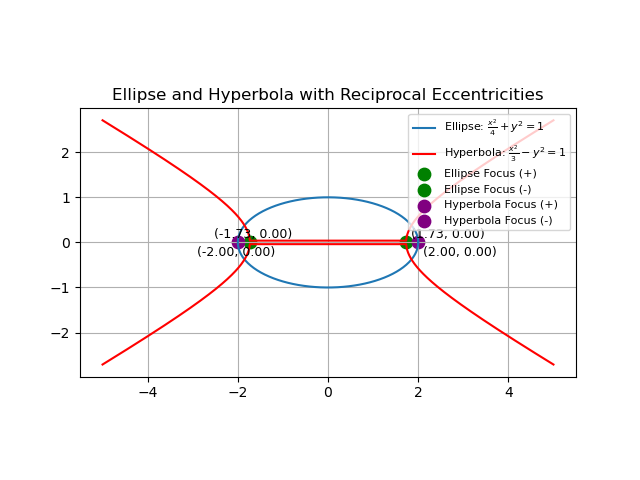
\includegraphics[height=0.5\textheight, keepaspectratio]{figs/Figure_1.png}
\end{figure}    
\end{frame}

\begin{frame}[fragile]
    \frametitle{C Code}
    \begin{lstlisting}
#include <math.h>
double ellipse_eccentricity(double a, double b) {
    return sqrt(1.0 - (b*b) / (a*a));
}
double hyperbola_eccentricity(double a, double b) {
    return sqrt(1.0 + (b*b) / (a*a));
}
double ellipse_focus(double a, double b) {
    return sqrt(a*a - b*b);
}
double hyperbola_focus(double a, double b) {
    return sqrt(a*a + b*b);
}
    \end{lstlisting}
\end{frame}
\begin{frame}[fragile]
    \frametitle{Python + C Code}
    \begin{lstlisting}
import ctypes
import numpy as np
import matplotlib.pyplot as plt

lib = ctypes.CDLL("./libconic.so")  

lib.ellipse_eccentricity.restype = ctypes.c_double
lib.ellipse_eccentricity.argtypes = [ctypes.c_double, ctypes.c_double]

lib.hyperbola_eccentricity.restype = ctypes.c_double
lib.hyperbola_eccentricity.argtypes = [ctypes.c_double, ctypes.c_double]

lib.ellipse_focus.restype = ctypes.c_double
lib.ellipse_focus.argtypes = [ctypes.c_double, ctypes.c_double]

lib.hyperbola_focus.restype = ctypes.c_double
lib.hyperbola_focus.argtypes = [ctypes.c_double, ctypes.c_double]

    \end{lstlisting}
\end{frame}
\begin{frame}[fragile]
    \frametitle{Python + C Code}
    \begin{lstlisting}
a_e, b_e = 2, 1
a_h, b_h = np.sqrt(3), 1

e_e = lib.ellipse_eccentricity(a_e, b_e)
e_h = lib.hyperbola_eccentricity(a_h, b_h)
c_e = lib.ellipse_focus(a_e, b_e)
c_h = lib.hyperbola_focus(a_h, b_h)

print(f"Eccentricities: e_E={e_e:.3f}, e_H={e_h:.3f}, Product={e_e*e_h:.3f}")
print(f"Ellipse focus distance: {c_e:.3f}, Hyperbola focus distance: {c_h:.3f}")

theta = np.linspace(0, 2*np.pi, 400)
x_ellipse = a_e * np.cos(theta)
y_ellipse = b_e * np.sin(theta)
focus1 = (c_e, 0)
focus2 = (-c_e, 0)



    \end{lstlisting}
\end{frame}
\begin{frame}[fragile]
    \frametitle{Python + C Code}
    \begin{lstlisting}
x_h = np.linspace(-5, 5, 2000)
x_h = x_h[np.abs(x_h) >= a_h]
y_h = np.sqrt((x_h**2 / a_h**2 - 1) * b_h**2)
focus_h1 = (c_h, 0)
focus_h2 = (-c_h, 0)
x_f, y_f = focus1
lhs = x_f**2 / a_h**2 - y_f**2 / b_h**2
print("Hyperbola LHS at ellipse focus =", lhs)
plt.plot(x_ellipse, y_ellipse, label=r'Ellipse: $\frac{x^2}{4} + y^2 = 1$')
plt.plot(x_h, y_h, 'r', label=r'Hyperbola: $\frac{x^2}{3} - y^2 = 1$')
plt.plot(x_h, -y_h, 'r')
plt.scatter(*focus1, color='green', s=80, label='Ellipse Focus (+)')
plt.scatter(*focus2, color='green', s=80, label='Ellipse Focus (-)')
plt.scatter(*focus_h1, color='purple', s=80, label='Hyperbola Focus (+)')
plt.scatter(*focus_h2, color='purple', s=80, label='Hyperbola Focus (-)')
plt.gca().set_aspect('equal')
plt.legend(fontsize=8, loc="upper right")
plt.title(fr"Ellipse & Hyperbola ($e_E={e_e:.3f}, e_H={e_h:.3f}$)")
plt.grid(True)
plt.savefig("/mnt/c/Users/bharg/Documents/backupmatrix/ee25btech11013/matgeo/8.4.16/figs/Figure_1.png")
plt.show()






    \end{lstlisting}
\end{frame}
\begin{frame}[fragile]
    \frametitle{Python + C Code}
    \begin{lstlisting}
plt.scatter(*focus_h2, color='purple', s=80, label='Hyperbola Focus (-)')
plt.gca().set_aspect('equal')
plt.legend(fontsize=8, loc="upper right")
plt.title(fr"Ellipse & Hyperbola ($e_E={e_e:.3f}, e_H={e_h:.3f}$)")
plt.grid(True)
plt.savefig("/mnt/c/Users/bharg/Documents/backupmatrix/ee25btech11013/matgeo/8.4.16/figs/Figure_1.png")
plt.show()

    \end{lstlisting}
\end{frame}

\begin{frame}[fragile]
    \frametitle{Python Code}
    \begin{lstlisting}
import numpy as np
import matplotlib.pyplot as plt

# Ellipse: x^2/4 + y^2 = 1

a_e, b_e = 2, 1
h_e, k_e = 0, 0

theta = np.linspace(0, 2*np.pi, 400)
x_ellipse = h_e + a_e * np.cos(theta)
y_ellipse = k_e + b_e * np.sin(theta)

# Ellipse foci
c_e = np.sqrt(a_e**2 - b_e**2)
focus1 = (h_e + c_e, k_e)
focus2 = (h_e - c_e, k_e)

# Hyperbola: x^2/3 - y^2 = 1
a_h = np.sqrt(3)
b_h = 1
h_h, k_h = 0, 0



    \end{lstlisting}
\end{frame}
\begin{frame}[fragile]
    \frametitle{Python Code}
    \begin{lstlisting}
x_h = np.linspace(-5, 5, 2000)
x_h = x_h[np.abs(x_h) >= a_h]  # valid domain
y_h = np.sqrt((x_h**2 / a_h**2 - 1) * b_h**2)

# Hyperbola foci (±2, 0)
c_h = 2
focus_h1 = (h_h + c_h, k_h)
focus_h2 = (h_h - c_h, k_h)

# Check if hyperbola passes through ellipse focus
x_f, y_f = focus1
lhs = x_f**2 / a_h**2 - y_f**2 / b_h**2
print("Hyperbola LHS at ellipse focus =", lhs)

plt.plot(x_ellipse, y_ellipse, label=r'Ellipse: $\frac{x^2}{4} + y^2 = 1$')
plt.plot(x_h, y_h, 'r', label=r'Hyperbola: $\frac{x^2}{3} - y^2 = 1$')
plt.plot(x_h, -y_h, 'r')

# Ellipse foci
plt.scatter(*focus1, color='green', s=80, label='Ellipse Focus (+)')
plt.scatter(*focus2, color='green', s=80, label='Ellipse Focus (-)')

    \end{lstlisting}
\end{frame}
\begin{frame}[fragile]
    \frametitle{Python Code}
    \begin{lstlisting}
plt.scatter(*focus_h1, color='purple', s=80, label='Hyperbola Focus (+)')
plt.scatter(*focus_h2, color='purple', s=80, label='Hyperbola Focus (-)')

plt.text(focus1[0]+0.1, focus1[1]+0.1, f'({focus1[0]:.2f}, {focus1[1]:.2f})', fontsize=9)
plt.text(focus2[0]-0.8, focus2[1]+0.1, f'({focus2[0]:.2f}, {focus2[1]:.2f})', fontsize=9)
plt.text(focus_h1[0]+0.1, focus_h1[1]-0.3, f'({focus_h1[0]:.2f}, {focus_h1[1]:.2f})', fontsize=9)
plt.text(focus_h2[0]-0.9, focus_h2[1]-0.3, f'({focus_h2[0]:.2f}, {focus_h2[1]:.2f})', fontsize=9)
plt.gca().set_aspect('equal')
plt.legend(loc = "upper right", fontsize=8) 
plt.grid(True)
plt.title("Ellipse and Hyperbola with Reciprocal Eccentricities")
plt.savefig("/mnt/c/Users/bharg/Documents/backupmatrix/ee25btech11013/matgeo/8.4.16/figs/Figure_1.png")
plt.show()


    \end{lstlisting}
\end{frame}

\end{document}

